\section{Results}
\label{sec:results}

\subsection{\texorpdfstring{\textcolor{blue}{Update Delivery (RQ1)}}{Update Delivery (RQ1)}}
\label{subsec:profiles}

\paragraph{\textcolor{blue}{How much of the traffic is update traffic}}
\textcolor{blue}{Update flows are a small part of what devices exchange while they update (Table~\ref{tab:funnel}, Figure~\ref{fig:composition}).
In our captures, 715 of 2,219 flows stay on the local network, e.g., tapo-c200's live video to the phone (86\% of its bytes), and most Internet flows serve streaming, telemetry, and time synchronization.
Where an image was transferred, however, the 250 update flows carry almost all bytes: 96 to 100\% for apple-tv, homepod, eufy-cam, xiaomi-cam, reolink-cam, and tapo-c100.
Separating the traffic also corrects individual observations: the only HTTP download of an Apple image in the apple-tv capture is a 5.5\,MB partial fetch of a 2013 restore image for an older Apple~TV model by a system component %(\texttt{TVDisplayAssistant}); 
the update itself arrived over TLS~1.3.}

\begin{figure}[!t]
    \centering
    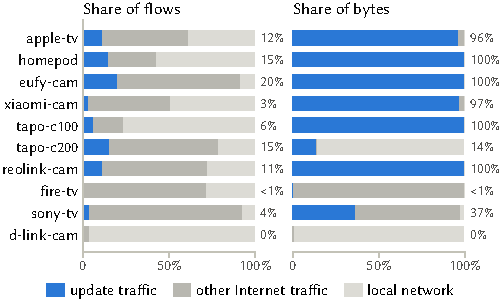
\includegraphics[width=\linewidth]{fig/traffic_composition.pdf}
    \caption{\textcolor{blue}{Share of flows and of bytes that are update traffic, per device, in our captures. Percentages give the update share.}}
    \Description{Two panels of horizontal 100-percent stacked bars, one bar per device. In the share of flows, update traffic is a small part for every device (0 to 20 percent). In the share of bytes, update traffic dominates for apple-tv, homepod, eufy-cam, xiaomi-cam, tapo-c100, and reolink-cam (96 to 100 percent), but not for tapo-c200 (14 percent), fire-tv, sony-tv, and d-link-cam.}
    \label{fig:composition}
\end{figure}

\paragraph{\textcolor{blue}{Delivery paths}}
\textcolor{blue}{Table~\ref{tab:profiles} summarizes how each device received its update, and Figure~\ref{fig:timelines} shows the exchanges of four devices over time.
Six devices fetched their image from vendor or cloud content delivery networks (Apple's own network; Amazon CloudFront and AWS for TP-Link and Eufy; Microsoft Azure and CDN77 for Xiaomi).
For five of them we also observed an update check or a metadata exchange with a separate server, and apple-tv additionally contacted Apple's installation-authorization service (\texttt{gs.apple.com}) before the download.
The update checks and the image transfer need not use the same protection: apple-tv retrieved its catalog and image over TLS~1.3 but most of its metadata and the authorization over TLS~1.2, and tapo-c200 polled TP-Link's device API over TLS for 23~minutes before downloading the image over HTTP.
reolink-cam contacted no update server: its desktop application pushed the image across the local network over a proprietary UDP protocol.}
Of the three devices that were up to date, fire-tv and sony-tv each opened a single update-check connection, and d-link-cam produced no update traffic at all.

\begin{figure*}[!t]
    \centering
    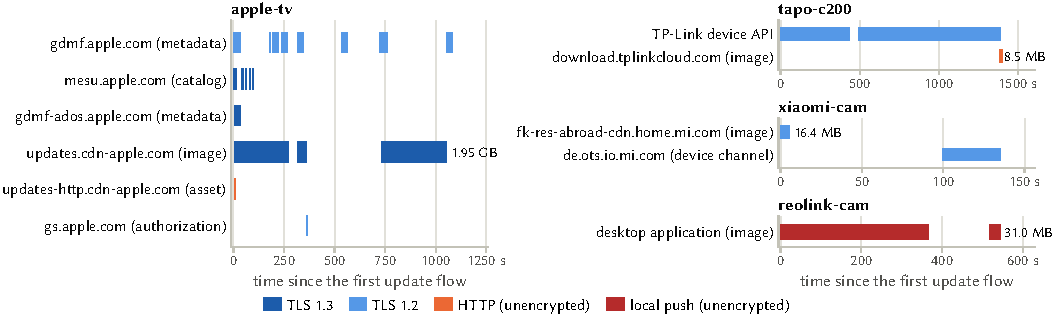
\includegraphics[width=\textwidth]{fig/update_timelines.pdf}
    \caption{\textcolor{blue}{Update exchanges over time for four devices. Each bar is one flow to an update server, from its first to its last packet, colored by how the flow is protected; labels give the size of image transfers. Short flows are widened to stay visible.}}
    \Description{Four timeline panels: apple-tv fills the left half, and tapo-c200, xiaomi-cam, and reolink-cam are stacked on the right. apple-tv: short TLS 1.2 metadata flows to gdmf.apple.com, TLS 1.3 catalog flows to mesu.apple.com, one authorization flow to gs.apple.com, and long TLS 1.3 image flows to updates.cdn-apple.com totalling 1.95 GB over about 1,000 seconds. tapo-c200: many short TLS 1.2 connections to TP-Link's device API for about 450 seconds, a long API connection, and at the end an 8.5 MB HTTP image download. xiaomi-cam: a 16.4 MB TLS 1.2 image download followed by a TLS 1.2 device-channel flow. reolink-cam: two unencrypted local-network flows from the desktop application, 31 MB in total.}
    \label{fig:timelines}
\end{figure*}

\begin{table*}[!t]
    \centering
    \color{blue}
    \caption{How the controlled devices received their updates. 1.2/1.3: TLS version; ECDHE-RSA-GCM: ECDHE key exchange, RSA authentication, AES-GCM (ciphersuite.info: \emph{secure}); TLS~1.3 suites are \emph{recommended}; static-RSA, PSK, and CBC suites are \emph{weak} (Table~\ref{tab:cipher_classes}). n/o: not observed. \textsuperscript{l}Likely update server (multi-purpose device API or unconfirmed check server). \textsuperscript{v}Vendor-published image of the installed firmware line. \textsuperscript{d}Per vendor documentation~\cite{apple-platform-security}.}
    \label{tab:profiles}
    \setlength{\tabcolsep}{2.4pt}
    \footnotesize
    \begin{tabular}{@{} l l l l l l >{\raggedright\arraybackslash}p{2.35cm} @{}}
        \toprule
        \textbf{Device} & \textbf{Firmware} & \textbf{Served from} & \textbf{Check / metadata} & \textbf{Image transfer} & \textbf{Server leaf certificate} & \textbf{Image protection} \\
        \midrule
        apple-tv    & 18.6 $\to$ 26.2       & Apple        & 1.3; 1.2 ECDHE-RSA-GCM                   & 1.3, 1.95\,GB & Apple CA, RSA-2048, 392\,d\textsuperscript{*} & signed, authorized per device\textsuperscript{d} \\
        homepod     & 18.6 $\to$ 26.2       & Apple        & 1.3                                      & 1.3, 1.1\,GB                & hidden by TLS~1.3                  & signed, authorized per device\textsuperscript{d} \\
        eufy-cam    & 2.1.0.2 $\to$ 2.3.1.6 & AWS          & 1.2 ECDHE-RSA-GCM\textsuperscript{l}     & 1.2 ECDHE-RSA-GCM, 19.7\,MB & public CA, RSA-2048, 397\,d        & unknown \\
        xiaomi-cam  & 3.5.1 $\to$ 4.0.9     & Azure, CDN77  & 1.2 PSK-CBC, no cert.\textsuperscript{l} & 1.2 ECDHE-RSA-GCM, 16.4\,MB & public CA, RSA-2048, 385\,d        & unknown \\
        tapo-c100   & 1.0.11 $\to$ 1.4.3    & CloudFront   & n/o                                      & HTTP, 6.7\,MB               & --                                 & signed \\
        tapo-c200   & 1.0.10 $\to$ 1.3.16   & AWS          & 1.2 static RSA-GCM\textsuperscript{l}    & HTTP, 8.5\,MB               & vendor CA, RSA-2048, 15\,y         & signed \\
        reolink-cam & 3.0.0 $\to$ 3.1.0     & desktop app (local) & n/o                                      & proprietary UDP, 31\,MB     & --                                 & no signature found \\
        fire-tv     & up to date            & AWS          & 1.2 ECDHE-RSA-GCM                        & --                          & public CA, RSA-2048, 340\,d        & signed\textsuperscript{v} \\
        sony-tv     & up to date            & AWS          & 1.2 ECDHE-RSA-CBC\textsuperscript{l}     & --                          & public CA, RSA-2048, 393\,d        & unknown \\
        d-link-cam  & up to date            & none observed & --                                       & --                          & --                                 & checksum only (CRC32)\textsuperscript{v} \\
        \bottomrule
        \multicolumn{7}{@{}l}{\textsuperscript{*}TLS~1.2 metadata servers; the TLS~1.3 connections hide the certificate.}
    \end{tabular}
\end{table*}

\paragraph{\textcolor{blue}{2019 baseline}}
\textcolor{blue}{In the retrospective traces, 15 device labels (13 models) contacted 12 confirmed update servers, as shown in Table~\ref{tab:retro}.
Although 97\% of the 2,497 update flows used TLS, four of the 15 labels sent some update traffic over HTTP: Apple~TV fetched signed assets and, once, its update catalog; the Samsung TV fetched firmware headers; the LG TV sent its update check; and the D-Link motion sensor queried its firmware server with its model, firmware version, and MAC address in the URL.}

\begin{table*}[!t]
    \centering
    \color{blue}
    \caption{Confirmed update servers in the 2019 Mon(IoT)r traces. All TLS connections negotiated TLS~1.2; suite abbreviations as in Table~\ref{tab:profiles}. \textsuperscript{a}echodot, t-echodot, echoplus, echospot, firetv, cloudcam. \textsuperscript{b}The thermostat also authenticates with a client certificate valid until 9999.}
    \label{tab:retro}
    \setlength{\tabcolsep}{4pt}
    \footnotesize
    \begin{tabular}{@{} l l l l l @{}}
        \toprule
        \textbf{Update server} & \textbf{Device labels} & \textbf{Protocol} & \textbf{Negotiated suite} & \textbf{Server leaf certificate} \\
        \midrule
        \texttt{softwareupdates.amazon.com} & six Amazon devices\textsuperscript{a} & TLS & ECDHE-RSA-GCM & DigiCert, RSA-2048, 336\,d \\
        \texttt{mesu.apple.com}             & appletv                     & TLS; once HTTP & ECDHE-ECDSA-GCM & Apple, EC P-256, 760\,d \\
        \texttt{gdmf.apple.com}             & appletv                     & TLS            & ECDHE-RSA-GCM   & Apple, RSA-2048, 760\,d \\
        \texttt{updates-http.cdn-apple.com} & appletv                     & HTTP (signed assets) & --        & -- \\
        \texttt{fw-update2.smartthings.com} & smartthings-hub, t-smartthings-hub & TLS     & ECDHE-RSA-GCM   & vendor CA, RSA-1024, 10\,y \\
        \texttt{awsota.linkplay.com}        & allure-speaker              & TLS            & ECDHE-RSA-GCM   & Amazon, RSA-2048, 396\,d \\
        \texttt{hub-updates.winkapp.com}    & wink-hub2                   & TLS            & ECDHE-RSA-GCM   & Comodo, RSA-2048, 730\,d \\
        \texttt{fwuprod.clouddevice.io}     & honeywell-thermostat        & TLS (mutual)   & ECDHE-ECDSA-GCM & vendor CA, EC P-256, 731\,d\textsuperscript{b} \\
        \texttt{otn.samsungcloudcdn.com}    & samsungtv-wired             & HTTP           & --              & -- \\
        \texttt{wrpd.dlink.com}, \texttt{api.dch.dlink.com} & dlink-mov    & HTTP           & --              & -- \\
        \texttt{snu.lge.com}                & lgtv-wired                  & HTTP           & --              & -- \\
        \bottomrule
    \end{tabular}
\end{table*}

\subsection{Channel Protection (RQ2)}
\label{subsec:channel}
Of the seven devices that downloaded an update, four received the image over TLS (apple-tv and homepod over TLS~1.3, eufy-cam and xiaomi-cam over TLS~1.2) and three without encryption.
tapo-c100 and tapo-c200 downloaded their images over HTTP from \texttt{tplinkcloud.com}; the request URLs encode model, hardware revision, and target version, and the images (6.7 and 8.5\,MB) can be recovered byte for byte.
reolink-cam's local push is the only update flow that protocol inspection leaves unclassified.
Its payload has a normalized Shannon entropy of 0.978, 
\textcolor{blue}{which Ren et al.'s ranges would label as likely encrypted, yet it contains UBI, uImage, and SquashFS signatures, and 96\% of sampled 64-byte chunks of the published v3.1 image occur verbatim in the stream: the image travels unencrypted and is merely compressed.
Entropy would thus have misclassified the one flow for which it was needed, so we base encryption status on protocol and content.}

\textcolor{blue}{Figure~\ref{fig:entropy} shows that this is not a corner case.
Per update flow, every TLS connection has a normalized entropy above 0.8, but so do all 14 unencrypted HTTP flows that carry images or signed assets (median 0.99) and the main local push (0.95): a compressed image is as incompressible as ciphertext.
Unencrypted update checks and metadata spread from 0.64 to 0.99 (median 0.73), because some carry binary or encoded content.
An entropy threshold would thus have labelled every unencrypted image transfer in both datasets as encrypted, which is why per-device entropy averages cannot show whether update channels are encrypted.}

\begin{figure}[!t]
    \centering
    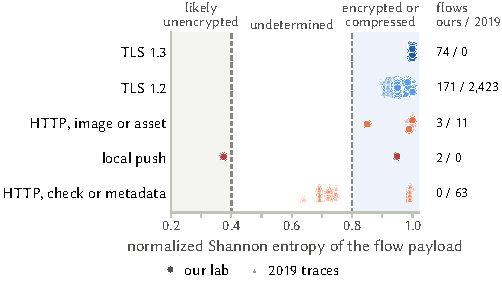
\includegraphics[width=\linewidth]{fig/entropy_by_channel.pdf}
    \caption{\textcolor{blue}{Normalized Shannon entropy of the payload of each update flow (server to device, first 2\,MB), grouped by how protocol inspection classifies the flow; dashed lines are the 0.4 and 0.8 ranges of Ren et al.~\cite{10.1145/3355369.3355577}. Unencrypted image transfers fall in the same range as TLS.}}
    \Description{Strip plot with five rows. TLS 1.3 flows (74, our lab) and TLS 1.2 flows (171 from our lab, 2,423 from 2019) all lie between 0.89 and 1.0. Unencrypted HTTP flows that carry images or assets (3 from our lab, 11 from 2019) lie between 0.85 and 1.0, in the same range. The main local-push flow lies at 0.95 and a small one at 0.37. Unencrypted HTTP update checks and metadata from 2019 (63 flows) lie between 0.64 and 0.99.}
    \label{fig:entropy}
\end{figure}

\paragraph{\textcolor{blue}{What unencrypted requests reveal}}
\textcolor{blue}{Table~\ref{tab:exposure} lists what the unencrypted update requests disclose to a passive observer.
The Tapo image URLs name the camera model, hardware version, region, and the firmware version about to be installed.
In 2019, the LG TV's update check (Base64-encoded, not encrypted) and the D-Link motion sensor's firmware query carried the installed firmware version together with the device's MAC address, a persistent identifier. The Apple~TV named its model, OS version, and build in the User-Agent of its HTTP asset downloads.
This suffices to single out devices that run a vulnerable version.
D-Link's newer upgrade interface, in contrast, encrypts its parameters at the application layer.
TLS hides such fields, but not which update server a device contacts, when, and how much it downloads: we identified every update flow from names sent in cleartext (\S\ref{subsec:attribution}), and a passive observer can do the same.
Nor does an encrypted update channel keep the version secret if other traffic reveals it: apple-tv, whose update traffic is all TLS, sent its model and OS build in the User-Agent of cleartext requests to an Apple identity service.}

\begin{table}[!t]
    \centering
    \color{blue}
    \caption{What unencrypted update requests reveal to a passive observer (values as observed; MAC addresses withheld).}
    \label{tab:exposure}
    \setlength{\tabcolsep}{3pt}
    \footnotesize
    \begin{tabular}{@{} l >{\raggedright\arraybackslash}p{1.55cm} >{\raggedright\arraybackslash}p{4.45cm} @{}}
        \toprule
        \textbf{Device} & \textbf{Request} & \textbf{Revealed} \\
        \midrule
        tapo-c100/c200 & image URL & model and hardware version (C100 v5, C200 v1), region, target version and build \\
        \addlinespace
        \multicolumn{3}{@{}l}{\emph{2019 traces}} \\
        appletv & User-Agent of asset downloads & model (AppleTV5,3), chip, installed OS version and build \\
        lgtv-wired & update check (Base64 XML) & platform, model code, installed firmware version, country, MAC address \\
        dlink-mov & firmware query URL & model (DCH-S150), hardware revision, installed firmware version, MAC address \\
        samsungtv-wired & firmware header URL & firmware line (platform and region), offered version \\
        \bottomrule
    \end{tabular}
\end{table}

\subsection{TLS Settings and Certificates (RQ2)}

\paragraph{Negotiated suites}
\textcolor{blue}{All 2,423 update connections in 2019 negotiated TLS~1.2 with ECDHE and AES-GCM (secure or recommended); no update server selected a weak or insecure suite.
The absence of TLS~1.3 reflects its early adoption after RFC~8446~\cite{rfc8446,holz2020tls13} rather than device limitations.
%: Apple~TV already offered TLS~1.3 suites in 2019, as shown in Figure~\ref{fig:offered}.
In our captures, the Apple devices use TLS~1.3 for catalog and image, and eufy-cam, xiaomi-cam's image server, and fire-tv's update check use ECDHE with AES-GCM.
Three channels negotiate weak suites: tapo-c200's device API selects static RSA (no forward secrecy) in all 144 connections, although the client also offers DHE suites; sony-tv's update check uses an ECDHE-RSA suite in CBC mode; and xiaomi-cam's device channel uses a pre-shared-key CBC suite without any certificate.}

\begin{figure}[!t]
    \centering
    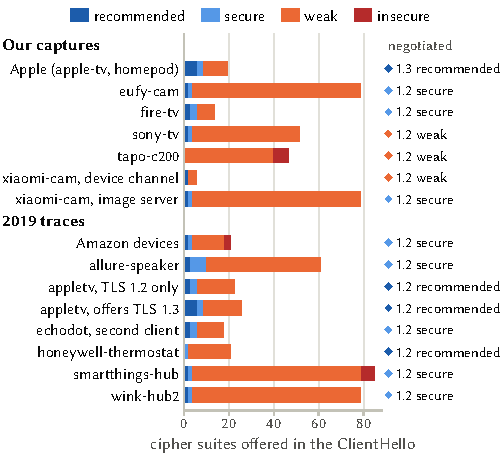
\includegraphics[width=\linewidth]{fig/offered_negotiated.pdf}
    \caption{\textcolor{blue}{Cipher suites offered per client configuration on update channels, by ciphersuite.info category, and the suite negotiated most often (diamond).}}
    \Description{Horizontal stacked bars, one per client configuration, showing how many offered suites fall into each category; most lists are dominated by weak suites, from about 10 to 80 suites long. A column on the right shows the negotiated suite with a colored diamond: TLS 1.3 recommended for Apple, secure or recommended TLS 1.2 suites for most other configurations, and weak suites for sony-tv, tapo-c200, and xiaomi-cam's device channel. tapo-c200, the 2019 Amazon devices, and the 2019 SmartThings hub also offer insecure suites.}
    \label{fig:offered}
\end{figure}

\paragraph{Offered suites}
\textcolor{blue}{Every client configuration offers weak suites, between 55\% (Apple, 11 of 20) and 95\% (eufy-cam and xiaomi-cam, 75 of 79) of its list, which mirrors library defaults rather than negotiated behavior (Figure~\ref{fig:offered}).
Insecure suites are rarer: tapo-c200's device-API client offers RC4 and single-DES suites (7 of 47) and no ECDHE suite at all, and in 2019 the Amazon devices and the SmartThings hub offered RC4.
None of these was ever negotiated, and because the Finished messages protect the offered list (\S\ref{sec:threat}), their presence is a hygiene issue rather than a downgrade path.}

\paragraph{Server certificates}
\textcolor{blue}{Figure~\ref{fig:lifetimes} shows the validity of the leaf certificates that update servers presented.
Leaves from public CAs and from Apple's CA are valid for 340-397 days in our captures and 336-760 days in 2019, within the CA/Browser Forum limits of the time~\cite{cabf-br}, and all use RSA-2048 or EC P-256 (112 or 128~bits).
The exceptions are CAs run by the vendors themselves, which these limits do not bind: TP-Link's device API presents a leaf valid for 15~years, and in 2019 SmartThings' firmware server presented an RSA-1024 leaf (80~bits) valid for ten years, while Honeywell's update server authenticated thermostats by client certificates valid until the year 9999.}

\begin{figure}[!t]
    \centering
    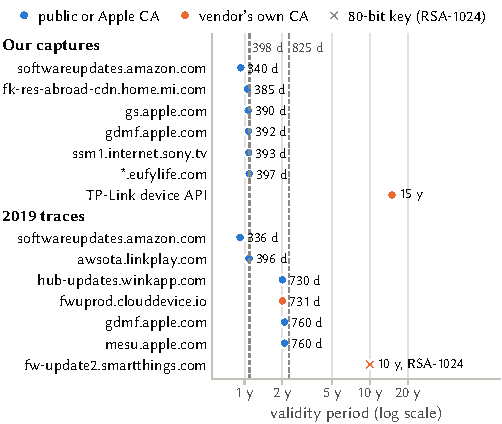
\includegraphics[width=\linewidth]{fig/leaf_lifetimes.pdf}
    \caption{\textcolor{blue}{Validity periods of the leaf certificates presented by update servers (log scale). Dashed lines: CA/Browser Forum limits for publicly trusted certificates (825 days until 2020, 398 days since).}}
    \Description{Dot plot with one row per update server, split into our captures and 2019 traces. Public and Apple certificates cluster between 336 and 760 days, at or below the limits. Two certificates from vendors' own authorities stand out: TP-Link's device API at 15 years, and SmartThings' firmware server in 2019 at 10 years with a 1024-bit RSA key.}
    \label{fig:lifetimes}
\end{figure}

\paragraph{\textcolor{blue}{Revocation}}
\textcolor{blue}{A long-lived certificate is a lasting risk mainly if it cannot be withdrawn after its key is compromised.
Table~\ref{tab:revocation} shows which revocation sources each leaf names, whether the client asks for a stapled OCSP response (visible in TLS~1.3 as well), and whether the device contacted any OCSP or CRL server during the capture.
The Apple devices, fire-tv, and in 2019 the Honeywell thermostat request stapling on every update connection, and where TLS~1.2 makes stapling visible, the server staples a response in 132 of 148 connections.
eufy-cam, xiaomi-cam, sony-tv, and the 2019 Amazon, LinkPlay, and Wink clients neither request stapling nor contact the responder that their public-CA leaf names.
The vendor-CA leaves are the extreme: TP-Link's 15-year leaf names only a revocation list, which tapo-c200 never fetched, and SmartThings' ten-year RSA-1024 leaf names no revocation source at all; the hubs contacted no OCSP or CRL server in 212 captures.}

\begin{table}[!t]
    \centering
    \color{blue}
    \caption{Revocation checking for update-server leaf certificates. \emph{Staple}: the client requests a stapled OCSP response. \emph{Lookup}: the device contacts an OCSP or CRL server during the capture. \textsuperscript{a}From Amazon's own CRL service (18 of 27 captures), not from the issuer of the leaf.}
    \label{tab:revocation}
    \setlength{\tabcolsep}{3pt}
    \footnotesize
    \begin{tabular}{@{} >{\raggedright\arraybackslash}p{2.45cm} l l l l @{}}
        \toprule
        \textbf{Server (clients)} & \textbf{CA, validity} & \textbf{In leaf} & \textbf{Staple} & \textbf{Lookup} \\
        \midrule
        Apple (apple-tv, homepod) & Apple, 390--392\,d & OCSP, CRL & all & apple-tv \\
        Amazon (fire-tv)          & public, 340\,d     & OCSP, CRL & all & no \\
        Eufy, Xiaomi, Sony        & public, 385--397\,d & OCSP, CRL & no & no \\
        TP-Link API (tapo-c200)   & vendor, 15\,y      & CRL       & no  & no \\
        \addlinespace
        \multicolumn{5}{@{}l}{\emph{2019 traces}} \\
        Apple (appletv)           & Apple, 760\,d      & OCSP, CRL & all & 7 of 28 \\
        Honeywell (thermostat)    & vendor, 731\,d     & OCSP, CRL & all & no \\
        Amazon (six devices)      & public, 336\,d     & OCSP, CRL & no  & other\textsuperscript{a} \\
        LinkPlay, Wink            & public, 396/730\,d & OCSP, CRL & no  & no \\
        SmartThings (hub)         & vendor, 10\,y      & none      & no  & no \\
        \bottomrule
    \end{tabular}
\end{table}

\textcolor{blue}{What does this mean for the NIST transition that disallows 112-bit strength for applying protection after 2030~\cite{NIST2020-SP800-57}?
A server's leaf certificate can be replaced on the server at any time, and public-CA leaves are replaced about yearly, so their RSA-2048 keys are not a lasting problem.
A leaf becomes one when it outlives the transition, as TP-Link's does (valid until 2036), or when the device can only trust its vendor's CA: then the trust anchor ships in the firmware, and changing it, or without revocation even withdrawing a compromised key, requires a firmware update, which devices that stop receiving updates before 2031 will not get.}

\subsection{\texorpdfstring{\textcolor{blue}{Image Protection (RQ2)}}{Image Protection (RQ2)}}
\label{subsec:image}
\textcolor{blue}{Figure~\ref{fig:channelimage} combines how each image reached the device with the protection inside it.
The Tapo images, delivered over HTTP, carry a signature block that requires TP-Link's private key, so an on-path adversary can read but not undetectably modify them, provided the device checks the signature.
Apple images are signed and authorized per device at installation time~\cite{apple-platform-security}, and Fire~TV update packages are signed.
The pushed reolink-cam image contains no signature that we could locate, and we could not reproduce its checksum, so this local push is the weakest combination we observed: an unencrypted transfer of an image without evident protection.
The published image of d-link-cam's installed firmware (DCS-5000L v1.05.02) is a uImage protected only by CRC32 header and data checksums; recomputing both after a modification yields an image that passes the format check, so its integrity would rest entirely on the channel.}

\begin{figure}[!t]
    \centering
    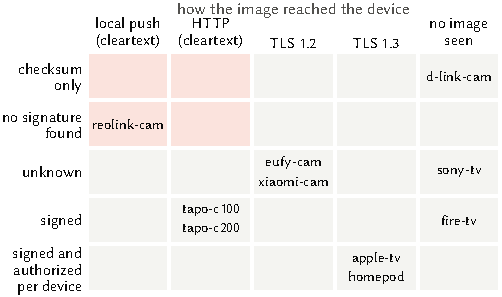
\includegraphics[width=\linewidth]{fig/channel_image.pdf}
    \caption{\textcolor{blue}{How each device's image reached it (columns) versus the protection inside the image (rows). In the shaded cells, an on-path attacker could alter the image without breaking any cryptography, provided the device installs it.}}
    \Description{A grid with five columns (local push unencrypted, HTTP unencrypted, TLS 1.2, TLS 1.3, no image seen) and five rows (checksum only, no signature found, unknown, signed, signed and authorized per device). reolink-cam sits in the shaded cell for a local unencrypted push without a signature; tapo-c100 and tapo-c200 are in HTTP and signed; eufy-cam and xiaomi-cam in TLS 1.2 and unknown; apple-tv and homepod in TLS 1.3 and signed with per-device authorization; d-link-cam, fire-tv, and sony-tv are in the no-image column.}
    \label{fig:channelimage}
\end{figure}

\subsection{\texorpdfstring{\textcolor{blue}{Attack Preconditions (RQ3)}}{Attack Preconditions (RQ3)}}
\label{subsec:preconditions}
\textcolor{blue}{Table~\ref{tab:preconditions} maps each weakness to the attack class it enables.
Only reconnaissance succeeds for a passive adversary without further requirements.
Every tampering path additionally requires that the device installs an image it cannot authenticate, which our data establish at the image level (reolink-cam, d-link-cam) or rule out at that level (Tapo, Apple, Fire~TV), but never at the level of device-side checking.
These are exposure statements: we neither attempted nor observed exploitation on the devices; the only manipulation we performed is the offline D-Link image modification above.}

\begin{table}[!t]
    \centering
    \color{blue}
    \caption{Observed weaknesses, the attacks they enable (CWE~\cite{mitre-cwe}; representative CVE~\cite{CVE_Program}), what the attacks require, and whether our data show the requirement to be met.}
    \label{tab:preconditions}
    \setlength{\tabcolsep}{2pt}
    \footnotesize
    \begin{tabular}{@{} >{\raggedright\arraybackslash}p{2.1cm} >{\raggedright\arraybackslash}p{2.05cm} >{\raggedright\arraybackslash}p{1.8cm} >{\raggedright\arraybackslash}p{2.05cm} @{}}
        \toprule
        \textbf{Weakness (where)} & \textbf{Enables} & \textbf{Requires} & \textbf{Met?} \\
        \midrule
        Unencrypted update check or download (Tapo; 2019: Apple~TV, D-Link, LG, Samsung) & reconnaissance of model and version; tracking by MAC address (CWE-319) & passive on-path $\mathcal{A}$ & yes (Table~\ref{tab:exposure}) \\
        \addlinespace
        Image over HTTP (tapo-c100, tapo-c200) & image substitution (CWE-494) & active $\mathcal{A}$; signature not checked & image signed; checking not observable \\
        \addlinespace
        Unencrypted local push (reolink-cam) & image substitution on the local network (CWE-494) & local access; no image protection & no signature found \\
        \addlinespace
        Checksum-only image (d-link-cam image) & forged image passes check (CWE-345) & unauthenticated delivery channel & no update observed \\
        \addlinespace
        Static RSA key exchange (tapo-c200 API) & decryption of recorded sessions; Bleichenbacher oracle (CWE-327; CVE-2017-13099) & server key compromise or vulnerable server & not observable; leaf valid 15~y \\
        \addlinespace
        CBC suites negotiated (sony-tv, xiaomi-cam) & padding oracle (CWE-327; CVE-2013-0169) & vulnerable implementation; active $\mathcal{A}$ & not observable \\
        \addlinespace
        RC4/DES offered (tapo-c200; 2019: Amazon, SmartThings) & RC4 biases, DES key search (CWE-327; CVE-2013-2566) & server selects them & no; never negotiated \\
        \addlinespace
        RSA-1024 server leaf (2019: SmartThings) & server impersonation (CWE-326) & factoring a 1024-bit key & below NIST minimum \\
        \addlinespace
        Long-lived leaf, revocation never checked (tapo-c200; 2019: SmartThings) & use of a stolen server key until the leaf expires (CWE-299) & key compromise; active $\mathcal{A}$ & not observable; valid 15 and 10~y \\
        \bottomrule
    \end{tabular}
\end{table}
